%%%%%%%%%%%%%%%%%%%%%%%%%%%%%%%%%%%%%%%%%%%%%%%%%%%%%%%%%%%%%%%%%%%%%%
% Overleaf (WriteLaTeX) Example: Molecular Chemistry Presentation
%
% Source: http://www.overleaf.com
%
% In these slides we show how Overleaf can be used with standard 
% chemistry packages to easily create professional presentations.
% 
% Feel free to distribute this example, but please keep the referral
% to overleaf.com
% 
%%%%%%%%%%%%%%%%%%%%%%%%%%%%%%%%%%%%%%%%%%%%%%%%%%%%%%%%%%%%%%%%%%%%%%
% How to use Overleaf: 
%
% You edit the source code here on the left, and the preview on the
% right shows you the result within a few seconds.
%
% Bookmark this page and share the URL with your co-authors. They can
% edit at the same time!
%
% You can upload figures, bibliographies, custom classes and
% styles using the files menu.
%
% If you're new to LaTeX, the wikibook is a great place to start:
% http://en.wikibooks.org/wiki/LaTeX
%
%%%%%%%%%%%%%%%%%%%%%%%%%%%%%%%%%%%%%%%%%%%%%%%%%%%%%%%%%%%%%%%%%%%%%%

\documentclass[hyperref={colorlinks,citecolor=blue,linkcolor=blue,urlcolor=blue}]{beamer}

% For more themes, color themes and font themes, see:
% http://deic.uab.es/~iblanes/beamer_gallery/index_by_theme.html
%
\mode<presentation>
{
  \usetheme{Madrid}       % or try default, Darmstadt, Warsaw, ...
  \usecolortheme{default} % or try albatross, beaver, crane, ...
  \usefonttheme{serif}    % or try default, structurebold, ...
  \setbeamertemplate{navigation symbols}{}
  \setbeamertemplate{caption}[numbered]
} 

\usepackage[english]{babel}
\usepackage[utf8x]{inputenc}
\usepackage{chemfig}
\usepackage[version=3]{mhchem}
\usepackage{tikz}
\usetikzlibrary{plotmarks}
\usepackage{pgfplots}
\usepackage{lineno}
\usepackage{tikz}
\usepackage{xcolor}
\usepackage{subcaption}
\usepackage{pgf}  
\usepackage{svg}
\usepackage{ragged2e}

\newlength\figureheight
\newlength\figurewidth
% \addtobeamertemplate{navigation symbols}{}{%
%     \usebeamerfont{footline}%
%     \usebeamercolor[fg]{footline}%
%     \hspace{5em}%
%     \insertframenumber/\inserttotalframenumber
% }

\setbeamertemplate{navigation symbols}{}
% \setbeamertemplate{footline}[frame number]{}
\setbeamertemplate{page number in head/foot}[totalframenumber]

% On Overleaf, these lines give you sharper preview images.
% You might want to `comment them out before you export, though.
\usepackage{pgfpages}
\pgfpagesuselayout{resize to}[%
  physical paper width=8in, physical paper height=6in]

% Here's where the presentation starts, with the info for the title slide
\title[]{Optimization and Prediction in Natural Gas Networks Using Graph Neural Networks and MPCC-Based Models}
\author{Cristian Alejandro Blanco Martínez}
\institute{Universidad Tecnológica de Pereira \\ 
Grupo de investigación Automática}
\date{\today}

\begin{document}

\begin{frame}
  \titlepage
\end{frame}




\begin{frame}{Energy Context \& Relevance of Natural Gas}
\justifying
Natural gas plays a crucial role in the global energy mix, offering a cleaner alternative to other fossil fuels by producing lower CO\textsubscript{2} emissions. It supports both industrial processes and electricity generation, acting as a reliable energy source in diverse contexts. 
\\ \\
In Colombia, natural gas is widely used across the residential, commercial, industrial, and thermal power sectors. Its importance becomes evident during dry seasons, when hydroelectric generation is reduced and thermal plants, fueled by natural gas, step in to maintain electricity supply.
\end{frame}

\begin{frame}{Operational Challenge in the Colombian Energy System}
\justifying
Colombia’s electricity supply relies heavily on hydroelectric plants, which are highly dependent on rainfall patterns. During dry seasons, reduced water availability forces the system to increase the participation of thermal plants powered by natural gas. 

This seasonal shift places significant operational stress on the gas transport network. 
% \begin{itemize}
%     \item More frequent re-optimizations of gas flows.
%     \item Rapid and accurate decision-making to ensure supply security.
% \end{itemize}

\begin{figure}[h]
    \centering
    \includegraphics[width=0.65\textwidth]{figures/hydro_vs_thermal.png}
    \caption{Variation in electricity generation mix between wet and dry seasons in Colombia.}
\end{figure}
\end{frame}


% These three lines create an automatically generated table of contents.
\begin{frame}{Motivation \& Problem Statement}
\justifying
\begin{itemize}
    \item \textbf{Large-scale natural gas networks} require solving complex optimization problems.
    \item Classical approaches are accurate but often \textbf{computationally expensive}.
    \item Increasing network size and operational constraints lead to:
    \begin{itemize}
        \item Long execution times
        \item Difficulty in real-time or near real-time decision making
    \end{itemize}
    \item Need for approaches that \textbf{preserve accuracy while reducing computation time}.
\end{itemize}
\end{frame}


\begin{frame}{Objectives}
\textbf{General Objective:}
\begin{itemize}
    \item Develop an optimization tool that integrates knowledge of the gas transportation network topology, a suitable approximation of the Weymouth equation and stochastic optimization techniques to address the gas transportation task taking into account the uncertainties related to hydroelectric generation and the growth of alternative energy sources.
\end{itemize}
\end{frame}

\begin{frame}{Objectives}
\textbf{Specific Objectives:}
\begin{itemize}
    \item Design a Graph Neural Networks-based approach of regression that integrates knowledge of natural gas network topology to reduce computational time for operation estimation.    
    \item Develop an optimization model for natural gas transportation systems that takes into account the Weymouth equation for reducing that reduces the approximation error in pipeline gas flow calculations.
    \item Develop a stochastic gas flow dispatch optimization strategy that quantifies the uncertainty in the objective variables and decision variables associated with the operation of the gas system taking into account the constraints of the transportation problem.
\end{itemize}
\end{frame}



%===========================================
% Chapter 2 — GNN Surrogate (CensNet) Overview
%===========================================
\section{Natural Gas System Prediction Using Graph Neural Networks}

%-------------------------------------------
% Slide 1: Motivation & Concept
%-------------------------------------------
\begin{frame}{Natural Gas System Prediction Using Graph Neural Networks}
    \begin{itemize}
        \item Traditional optimizers are \textbf{accurate but slow} for large-scale or real-time scenarios.
        \item Gas networks are inherently \textbf{graphs}: nodes = wells, users, storage; edges = pipelines, compressors.
        \item GNNs exploit \textbf{topology-aware learning} for faster prediction.
        \item \textbf{Goal:} Achieve near-optimizer accuracy with runtime reduction.
    \end{itemize} 
\end{frame}

%-------------------------------------------
% Slide: CensNet Architecture
%-------------------------------------------

\begin{frame}{CensNet Layers: Integrating Node \& Edge Features}
\footnotesize
\textbf{Motivation:}  
Traditional GCNs focus mainly on \textit{node features} and ignore \textit{edge features}, missing part of the graph’s information.

\medskip
\textbf{CensNet innovation:}
\begin{itemize}
    \item Alternates between \textbf{node layers} and \textbf{edge layers}.
    \item Each layer type updates its own features while using information from the other:
    \begin{itemize}
        \item \textbf{Node layer:} Node embeddings are updated using both node adjacency and transformed edge features.
        \item \textbf{Edge layer:} Edge embeddings are updated using edge adjacency and transformed node features.
    \end{itemize}
    \item Uses an \textit{incidence matrix} \( \mathbf{T} \) to switch between node and edge domains.
\end{itemize}

\medskip
\textbf{Benefits:}
\begin{itemize}
    \item Captures both \textit{structural} (adjacency) and \textit{relational} (edge) information.
    \item Enhances long-range dependencies through alternating propagation.
\end{itemize}
\end{frame}

\begin{frame}{Mathematical Structure of CensNet Layers}
\footnotesize
\textbf{Node layer propagation:}
\[
\mathbf{H}^{(l+1)}_v = \sigma\left(
\mathbf{T} \Phi(\mathbf{H}^{(l)}_e \mathbf{p}_e) \mathbf{T}^\top 
\odot \tilde{\mathbf{A}}_v \mathbf{H}^{(l)}_v \mathbf{W}_v
\right)
\]
\textbf{Edge layer propagation:}
\[
\mathbf{H}^{(l+1)}_e = \sigma\left(
\mathbf{T}^\top \Phi(\mathbf{H}^{(l)}_v \mathbf{p}_v) \mathbf{T} 
\odot \tilde{\mathbf{A}}_e \mathbf{H}^{(l)}_e \mathbf{W}_e
\right)
\]

\medskip
\textbf{Key components:}
\begin{itemize}
    \item \( \tilde{\mathbf{A}}_v, \tilde{\mathbf{A}}_e \): normalized adjacency matrices (nodes/edges).
    \item \( \mathbf{T} \): incidence matrix mapping between node and edge domains.
    \item \( \Phi(\cdot) \): diagonal scaling from projected features.
    \item \( \odot \): element-wise filtering of adjacency by feature-derived weights.
\end{itemize}

\medskip
\textbf{Core idea:} Information “switches” between node and edge spaces at each step, enriching representations.
\end{frame}

\begin{frame}{CensNet-based Model Architecture}
\footnotesize
\justifying
    \centering
    \resizebox{0.9\textwidth}{!}{%
        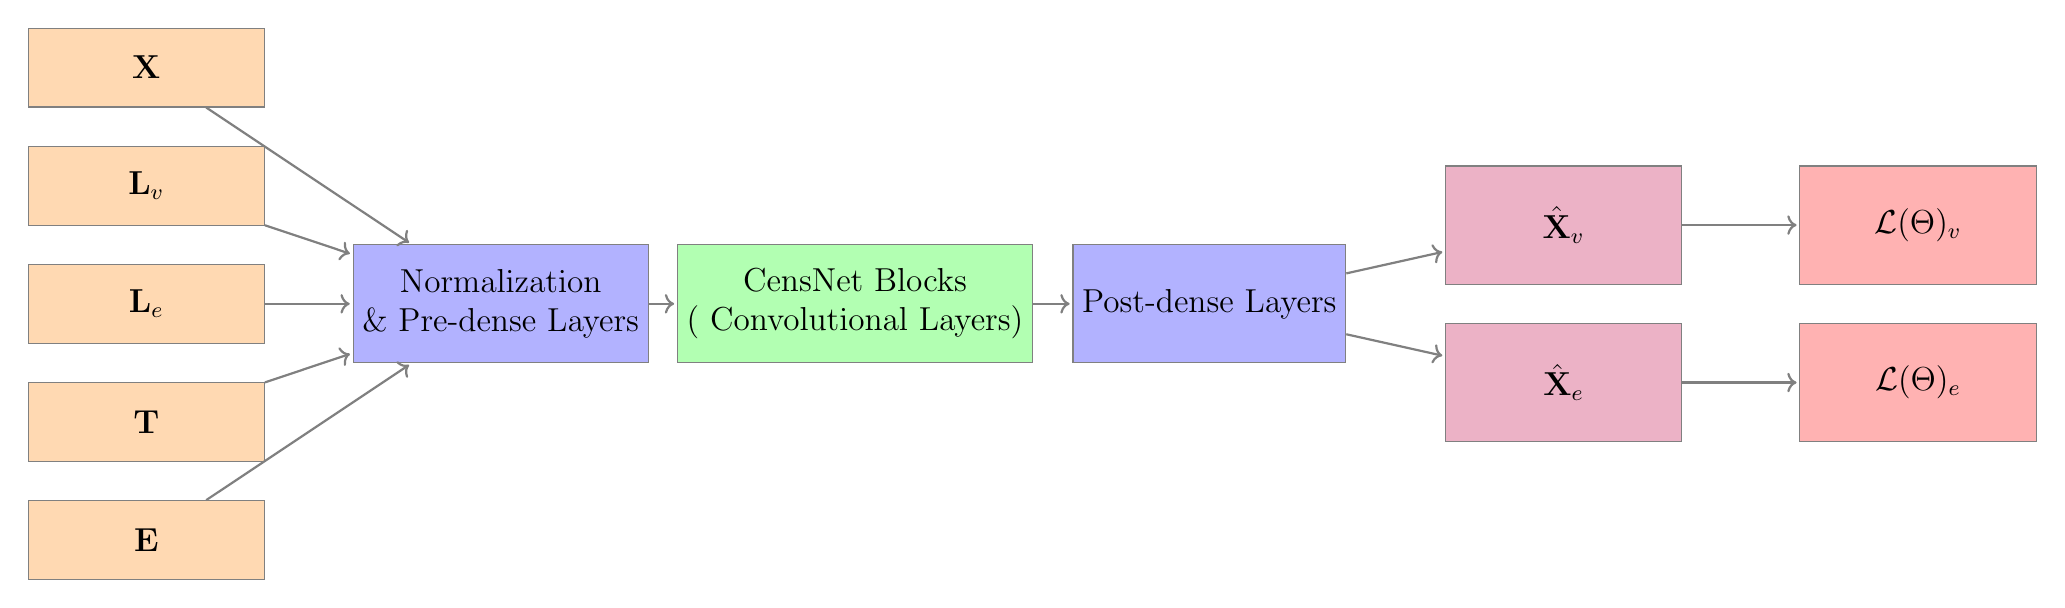
\begin{tikzpicture}[shorten >=1pt, ->, draw=black!50, node distance=1.5cm and 3.5cm, align=center]

    % Styles
    \tikzstyle{input} = [rectangle, draw, fill=orange!30, minimum width=3cm, minimum height=1cm, text centered, font=\large]
    \tikzstyle{dense} = [rectangle, draw, fill=blue!30, minimum width=3cm, minimum height=1.5cm, text centered, font=\large]
    \tikzstyle{conv} = [rectangle, draw, fill=green!30, minimum width=3cm, minimum height=1.5cm, text centered, font=\large]
    \tikzstyle{output} = [rectangle, draw, fill=purple!30, minimum width=3cm, minimum height=1.5cm, text centered, font=\large]
    \tikzstyle{loss} = [rectangle, draw, fill=red!30, minimum width=3cm, minimum height=1.5cm, text centered, font=\large]
    \tikzstyle{arrow} = [->, thick]

    % Input Layer
    \node[input] (node_features) at (0,0) {\(\mathbf{X}\)}; % Node Features
    \node[input] (node_laplacian) [below of=node_features] {\(\mathbf{L}_v\)}; % Node Laplacian
    \node[input] (edge_laplacian) [below of=node_laplacian] {\(\mathbf{L}_e\)}; % Edge Laplacian
    \node[input] (incidence_matrix) [below of=edge_laplacian] {\(\mathbf{T}\)}; % Incidence Matrix
    \node[input] (edge_features) [below of=incidence_matrix] {\(\mathbf{E}\)}; % Edge Features

    % Normalization and Pre-dense Layer
    \node[dense] (norm_pre_dense) [right of=edge_laplacian, xshift=3cm] {Normalization \\ \& Pre-dense Layers};

    % Convolutional Layers
    \node[conv] (conv_layers) [right of=norm_pre_dense, xshift=3cm] { CensNet Blocks \\ ( Convolutional Layers)};

    % Post-dense Layer
    \node[dense] (post_dense) [right of=conv_layers, xshift=3cm] {Post-dense Layers};

    % Outputs
    \node[output] (node_output) [right of=post_dense, xshift=3cm, yshift=1cm] {\(\hat{\mathbf{X}}_v\)}; % Node Predictions
    \node[output] (edge_output) [right of=post_dense, xshift=3cm, yshift=-1cm] {\(\hat{\mathbf{X}}_e\)}; % Edge Predictions

    % Losses
    \node[loss] (node_loss) [right of=node_output, xshift=3cm] {\(\mathcal{L}(\Theta)_v\)};
    \node[loss] (edge_loss) [right of=edge_output, xshift=3cm] {\(\mathcal{L}(\Theta)_e\)};

    % Arrows
    \draw[arrow] (node_features) -- (norm_pre_dense);
    \draw[arrow] (node_laplacian) -- (norm_pre_dense);
    \draw[arrow] (edge_laplacian) -- (norm_pre_dense);
    \draw[arrow] (incidence_matrix) -- (norm_pre_dense);
    \draw[arrow] (edge_features) -- (norm_pre_dense);

    \draw[arrow] (norm_pre_dense) -- (conv_layers);

    \draw[arrow] (conv_layers) -- (post_dense);

    \draw[arrow] (post_dense) -- (node_output);
    \draw[arrow] (post_dense) -- (edge_output);

    \draw[arrow] (node_output) -- (node_loss);
    \draw[arrow] (edge_output) -- (edge_loss);

\end{tikzpicture}

%
    } 

\textbf{Inputs:} Encapsulate both physical attributes and topological information of the gas network:
        \begin{itemize}
            \item Node features ($\mathbf{X}$): pressures, injections, withdrawals, demand forecasts.
            \item Node Laplacian ($\mathbf{L}_v$) and Edge Laplacian ($\mathbf{L}_e$): encode structural connectivity and enable topology-aware learning.
            \item Edge features ($\mathbf{E}$): capacities, lengths, compressor ratios.
            \item Incidence matrix ($\mathbf{T}$): explicit mapping between nodes and edges.
        \end{itemize} 
\end{frame}


\begin{frame}{CensNet-based Model Architecture}   
\footnotesize
    \begin{itemize} 
        \item \textbf{Processing:}
        \begin{itemize}
            \item Normalization and pre-dense layers transform heterogeneous inputs into a common latent space.
            \item \emph{CensNet convolutional blocks} perform message passing on both node and edge domains, enabling simultaneous learning of flow patterns and interactions.
            \item Post-dense layers refine features for prediction.
        \end{itemize}
        
        \item \textbf{Outputs:}
        \begin{itemize}
            \item Node-level injected flows ($\hat{\mathbf{X}}_v$) — predicted gas supply/demand at each node.
            \item Edge-level transported flows ($\hat{\mathbf{X}}_e$) — predicted flow rates in each pipeline.
        \end{itemize}
        
        \item \textbf{Training:} Node and edge predictions are penalized separately using task-specific loss terms, ensuring both accuracy and physical consistency.
    \end{itemize}

\end{frame}
%-------------------------------------------
% Slide 3: Loss Functions
%-------------------------------------------
\begin{frame}{Task-Dependent Loss Functions}
    \begin{itemize}
        \item Regression task $\Rightarrow$ Regularized MSE loss:
        \[
            \mathcal{L}(\Theta) = \sum_{r=1}^{R} \| Y_r - \hat{Y}_r \|^2_2 + \lambda \|\Theta\|_p
        \]
        \item Supports:
        \begin{itemize}
            \item \textbf{Nodal losses} – Injected flows
            \item \textbf{Edge losses} – Transported flows
            \item \textbf{Gas balance} – Physical consistency
        \end{itemize}
        \item Regularization avoids overfitting.
    \end{itemize}
\end{frame}

%-------------------------------------------
% Slide 4: Datasets
%-------------------------------------------
\begin{frame}{Test Systems}
    \begin{columns}[T]
        \begin{column}{0.6\textwidth}
            \begin{itemize}
                \item \textbf{8-node network:} Small-scale testbed.
                \item \textbf{63-node network:} Realistic Colombian gas infrastructure.
                \item Data: Generated via optimization model \eqref{eq:obj_func_linear_gas} with physical constraints \eqref{eq:well_limits}–\eqref{eq:gas_balance}.
            \end{itemize}
        \end{column}
        \begin{column}{0.4\textwidth}
            \centering
            % \includegraphics[width=\linewidth]{figs/network_maps.pdf} % <-- placeholder path
            \captionof{figure}{Case study networks.}
        \end{column}
    \end{columns}
\end{frame}

%-------------------------------------------
% Slide 5: Runtime vs Accuracy
%-------------------------------------------
\begin{frame}{Runtime vs Accuracy Trade-off}
    \begin{columns}[T]
        \begin{column}{0.55\textwidth}
            \begin{itemize}
                \item Optimizer: High accuracy, high runtime.
                \item CensNet: Comparable accuracy, much faster inference.
                \item Statistical validation: t-test confirms no significant loss in accuracy (p-values $\ll 0.05$).
            \end{itemize}
        \end{column}
        \begin{column}{0.45\textwidth}
            \centering
            % \includegraphics[width=\linewidth]{figs/runtime_accuracy_plot.pdf} % <-- placeholder path
            \captionof{figure}{Prediction accuracy vs computation time.}
        \end{column}
    \end{columns}
\end{frame}

\end{document}
